\documentclass[a4paper,10pt]{report}

\usepackage[utf8]{inputenc}
\usepackage{hyperref}
\hypersetup{
    colorlinks=true,
    linkcolor=black,
    filecolor=magenta,      
    urlcolor=black,
}
\usepackage{graphicx}
\usepackage[font=footnotesize,labelfont=bf]{caption}
\graphicspath{ {figures/} }

\title{Reconstruction of a macro-complex using interacting subunits}
\author{Lydia Fortea \and Juan Luis Melero}
\date{}

\pdfinfo{%
  /Title    (Reconstruction of a macro-complex using interacting subunits)
  /Author   (Lydia Fortea and Juan Luis Melero)
  /Creator  ()
  /Producer ()
  /Subject  (Structural Bioinformatics and Introduction to Python)
  /Keywords (modelling, reconstruction, macro-complex, structural alignment, structural bioinformatics)
}

\begin{document}
\maketitle
\tableofcontents{}

\chapter{Background}

The aim of the project is to reconstruct a marco-complex having only the pair interacting chains, using a standalone program created by ourselves.
The program we created is based on several bioinformatic features, including structural superimposition and sequence alignment, among others.

\section{Protein-Protein Interaction and Complexes}

An important point of the project is understanding the Protein-Protein Interaction and Complexes. In the quaternary structure of a protein, there are more than one separated chains of proteins that interacti between them.
The interaction of these chains can involve a lot of intermolecular bounds, such as hydrogen bounds, electrostatic interactions, pi stacking, cation-pi interaction, etc. This diversity of interactions makes the protein-protein interaction
very common in order to stabilized the molecule and generate a biological function.\\\\
The whole structure, where two or more chains are combined and have one or different functions, is called a complex. The formation of a complex can be made by protein-protein interaction only or nucleotides (DNA or RNA) can also be part of a complex if there is DNA-protein or RNA-protein interactions.\\\\
Focusing on the project, having the protein-protein interaction by pairs, we want to reconstruct the whole macro-complex.

\section{Sequence Alignment}

Pairwise sequence alignment is done for several reasons. One of them is because we want to compare the chains from the same interacting file to know if it is a homodimer or a heterodimer. Another reason is to compare different interacting files, in order to know if they are the same pair of interacting chains or they are different. The last one, is to know which chains must be superimposed, in case the interacting chains are different heterodimers (see section Modules and Packages, subsection Homodimers and Heterodimers).

\section{Structural superimposition}



We cannot assume that the protein-protein interacting pairs are well oriented in the space. Therefore, in order to give to each part the correct orientation, we do a structural superimposition. Structural superimposition allows us to put the chains in the correct spatial orientation, and we use sequence alignment to know which chains must be superimposed. With superimposition, all the chains will be well positioned. 



\chapter{Algorithm and Program}


\section{Inputs and Outputs}

\subsection{Input files}

The program takes interacting pair chains for building the macro-complex. However, in the command line, the input must be one of the following:

\begin{itemize}
 \item The list of PDB file names which contains the interacting pair chains.
 \item A directory that contains all the PDB files of interacting pair chains.
 \item By default, if no input is indicated, it takes the current directory as input, and takes all the PDB files as interacting pair chains.
\end{itemize}

\noindent
Input files must be all in the directory specified in the arguments or in the current directory by default. The program will read all the PDB files, so it is necessary that all the PDB files in the working directory are the subunits of the macrocomplex and nothing else.

\subsection{Output file}

The output file will be one PDB file in which there will be the coordinates of the atoms of the macro-complex. The output file will be located in the directory specified in the arguments. 
Depending on the inputs (homodimer, heterodimer or mixed), the output will have different names in the current directory (homodimer\_complex.pdb, heterodimer\_complex.pdb or homodimer\_heterodimer\_complex.pdb if mixed). If the current directory is the same in which there are the input files, be careful if you want to exercute the program twice or more times at the same time, since it will take the output file also as one of the input files.


\section{Modules and Packages}

\textit{Biopython} is the principal package used, as well as \textit{sys}, \textit{os}, \textit{re}, \textit{argparse}, \textit{subprocess} and the self-created modules \textit{homodimers} and \textit{heterodimers}. 

\subsection{Biopython}

Biopython is the main open-source collection of tools written in Python to work with biological data. From Biopython we take the following subpackages:

\begin{itemize}
 \item Bio.PDB, to work with PDB files. From Bio.PDB we use the following subpackages:
 \begin{itemize}
  \item PDBParser, to parse PDB files and obtain Structure Objects to work.
  \item CaPPBuilder, to create the sequences taking into account Ca-Ca distance.
  \item PDBIO, to save the structures into a PDB file.
  \item Superimpose, to execute structural superimposition between structures.
 \end{itemize}
 \item Bio.pairwise2, to align protein sequences one by one
\end{itemize}


\subsection{sys}

Sys package is the System-specific parameters and functions. This package is used to read the arguments in the command line (sys.argv) and to have access to the three channels of communication with the computer: the \textit{standard in} (sys.stdin), the \textit{standard out} (sys.stdout) and the \textit{standard error} (sys.stderr).

\subsection{os}

Os package is the Miscellaneous operating system interfaces. With this package, the program can access synonimous commands of the shell, allowing the program to, for example, change working directory (\textit{cd} in shell, \textit{os.chdir} in python). 
This package is usefull to call command lines from the system but without consuming as much CPU.

\subsection{re}

Re package in the Regular expression operations package. It allows to work with regular expressions with python. In the program, it is used to find PDB and FASTA files, searching the extension of FASTA (.fa, .fasta) and PDB (.pdb) as regular expression at the end of the files.


\subsection{argparse}

Argparse package is the Parser for command-line options, arguments annd sub-commands. This packages allows to include the options for the user. The options included in the program are described in section \textit{Options and Arguments}.

\subsection{subprocess}

Subprocess package is the subprocess manager that allows us to use bash and shell commands. In our program is used to call Chimera Software if the option -vz, -{}-visualize (see section Options and Arguments) is active.

\subsection{Homodimers, Heterodimers and Common Functions}

Homodimers and Heterodimers are self-created modules which analyze the structures depending on the input files. If the pair of chains in the interacting files are the same (A-A), then it is considered \texitit{homodimer}. If the pair of chains in the interacting files are different (A-B) but all the files contain this heterodimer (files are A-B, A-B...), then it is considered \textit{repeated heterodimer}. Finally, if the pair of chains in the interacting files are different and all interacting files are different (A-B, B-C...), then it is considered \textit{heterodimer}. For homodimers and repeated heterodimers, homodimers module is used. For heterodimers, heterodimers module is used.

\subsubsection{Homodimers module}

Homodimers module (\textit{homodimers.py}) contains two functions:

\begin{itemize}
 \item get\_structure\_homodimer, that is used when the input files are all homodimers
 \item get\_structure\_mix, that is used when the input files are homodimers and heterodimers.
\end{itemize}

\noindent
Both functions are explained in section Functions.

\subsubsection{Heterodimers module}

Heterodimers module (\textit{heterodimers.py}) contains two function:

\begin{itemize}
 \item align\_sequences\_heterodimers
 \item superimpose\_structures\_heterodimers
\end{itemize}

\noindent
Both functions are explained in section Functions.

\subsubsection{Common Functions Module}

Common functions module (\textit{common\_functions.py}) is a module that contains general functions that will be used during the program. This functions are:

\begin{itemize}
 \item get\_sequence
 \item seq\_comparison
 \item chains\_comparison
 \item temp\_structure
 \item clash\_identifier
 \item save\_complex
\end{itemize}

\noindent
All these functions are explained in section Functions.

\section{Functions}

In the program there are a lot of functions that will be used during the process of building the macro-complex. These functions are explained below.

\subsection{get\_input}

This function handles the input argument. It uses regular expressions to find those files ended with ".pdb" and puts them into a list. If the input is a list of files, then it puts them directly into a list. The function returns a list that is the PDB interacting files that will be used to build the complex.

\subsection{get\_name\_structure}

This function uses regular expressions to return the filename of the PDB file.

\subsection{common\_functions.get\_sequence}

This function deletes heteroatoms and returns the sequence of the proteins with more than 40 aminoacids (to avoid ligands). It uses CaPPBuilder package.

\subsection{common\_functions.seq\_comparison}

This function is used to find identical sequences. It performs a pairwise sequence alignment and if the percentage of identity (\%id) is greater than 0.95 it returns True, else, it returns False. It uses Bio.pairwise2 package to make the alignments.

\subsection{common\_functions.chains\_comparison}

This function compares the chains of the interacting pairs and returns Frue if they are the same or False if they are different. It uses seq\_comparison function.

\subsection{get\_pdb\_info}

This function analyze all the PDB files from the input. It extracts and compare the structures and their sequences in order to know if we have heterodimers o homodimers. It returns the pairwise interactions, the homodimer interactions and the heterodimer interactions.

\subsection{common\_functions.temp\_structure}

This function creates a temporary structure with the interactions. It returns the built structure.

\subsection{common\_functions.clash\_indentifier}

This function checks the final structure if there were any clash. It returns True if there are clashes or False if there is not any clash. If there were any clash, the chain is not added.

\subsection{common\_functions.save\_complex}

This function saves the structure into a PDB file. It return nothing, but creates the PDB output file. This function uses Bio.PDBIO package.

\subsection{heterodimers.align\_sequences\_heterodimers}

This function extracts all the sequences of the chains and aligns them with pairwise alignment and stores the percentage of identity (\%id). Those chains with a \%id greater than 99\% are assumed to be the same and then, they are going to be superimposed. 

\subsection{heterodimers.superimpose\_structures\_heterodimers}

This function is used to superimpose different structures. The chains that will be superimposed are those with the best alignment from \textit{heterodimer.align\_\\sequences\_heterodimers}. 
We do the superimposition taking one chain as reference chain and the other as moving chain. Then the coordinates are updated and the reference chain is deleted in order not to have repeated superimposed chains. 
After the superimposition, one of the chains superimposed is removed not to have repeated chains in the structure. It returns the structures superimposed.

\subsection{homodimers.get\_structure\_homodimer}

This function is called when the input files are homodimers or repeated heterodimers. It superimposes the structures, taking one as reference and correcting the coordinates, and afterwards eliminates one of the superimposed chains not to have redundancies. It returns the built structure.

\subsection{homodimers.get\_structure\_mix}

This function is called when there is a mix between homodimers and heterodimers in the input files. First, it aligns and superimposes homodimers like function \textit{homodimers.get\_structure\_homodimer} and after that it adds heterodimers interactions, superimposing them like heterodimers module. It returns the built structure.


\section{Workflow}

First of all, we take the input files provided by the user using \textit{get\_input} function. We extract the information from these PDB files to know if we are dealing with homodimers (A-A interactions), repeated heterodimers (A-B, A-B...) or distinct heterodimers (A-B, B-C...). To do that, we use \textit{get\_pdb\_info} function.\\\\
If the interactions are homodimers (A-A), repeated heterodimers (A-B, A-B...) or a mix of homodimers and heterodimers, then we use the standalone module \textit{homodimers.py}. If the interactions are distinct heterodimers (A-B, B-C...), then we use the module \textit{heterodimers.py}. You can see the workflow of each module in section \textit{Modules and Packages}, subsection \textit{Homodimers and Heterodimers}.\\\\
Finally, the program creates and saves a PDB file with the final structure using \textit{temp\_structure} and \textit{save\_complex} functions. If the option visualize (-vz, -{}-visualize) is activated, it opens the PDB output file with chimera (see section \textit{Options and Arguments} for requirements of this option).


\section{Restrictions and Limitations of the Program}


For heterodimers, one of the main restrictions is that all chains must be able to be followed. That is, we must be able to build a path joining all the subunits (A-B, B-C, C-D...). If it is not like that (A-B, C-D... for example), the program will crash. This is because one chain will be used as reference chain, and the other as moving chain. If it only appears once, then it is not possible to build the structure.\\\\
There are many problem handling homodimer interactions or heterodimer interaction. The main one is that structural superimposition is not useful to rebuild the protein. Moreover, we do not consider the stoichiometry (how many repetitions there are) and we assume that, the same interaction is only once and, if it were repeated, the user will provide it again. We could ask for the stoichiometry to the user to avoid this problem, and change the code to handle this.\\\\
The program does not work for protin-nucleotide interaction. To do this, we should analyse also nucleotide structures in PDB and change the code to work with nucleotides.\\\\
The program does not check if the PDB files are well-formatted. If there were any error in the input files, it could rise an error at some point of the program or create an output with the wrong-formatted data that, obiously, will not correspond to the correct macro-complex. If we knew what are the most typical errors or how a PDB cannot be well-formatted, we could rise an error before the script.\\\\
The program does not take into account proteins with less than 40 aminoacids. This is made to avoid peptide ligands. Therefore, small proteins will not be considered in the program. We could solve this if we knew the nature of the PDB structure, if ligand or protein.\\\\
We only create one model. There program could generate many models and compare them (e.g. analysing the energy) and then choose the best structure. Moreover, there is no evaluation of the quality of the model and the structure created.\\\\
If different chains have the same name, they are added as new structures. This is done because Chimera has problems recognizing differet chains with the same name. Therefore, although they could be the same chain, the name is changed.\\\\


\chapter{How to use the program}

\section{Requirements}

The main program requires for \textit{Biopython} package and auxiliary modules \textit{homodimers.py}, \textit{heterodimers.py} and \textit{common\_functions.py}, as well as all preinstalled Python packages indicated in \textit{Modules and Packages} section.

\section{Options and Arguments}

In the program the following arguments are available:

\begin{itemize}
 \item -i, -{}-input; it takes the directory as input. By default, it takes the current directory.
 \item -o, -{}-ouput; it takes the directory and the filename of the PDB file. By default, it creates a file called \textit{output.pdb} in the current directory.
 \item -s, -{}-sequence; it takes the directory and the filename of the FASTA file in which there is the sequence of the macro-complex. By default, it takes de value \textit{None} and runs the program with default parameters.
 \item -v, -{}-verbose; if this option is active, it prints the log to the standard error. 
 \item -vz, -{}-visualize; if this option is active, at the end of the script it opens the output file with Chimera. It will only work if Chimera is installed and the software is in \texttt{/usr/bin/chimera}, which is the path that the program calls Chimera Software.
\end{itemize}

All options are not forced to be, but it is highly recommended to use them, specially those related to the input/ouput files.

\section{Logging}

Activating the option for verbose (-v, -{}-verbose), it prints to the standard error the log of the program. The point that are verbosed and the message if it is all right are the followings:

\begin{itemize}
 \item Warning for files that were not analyzed because they were wrong.
 \item Print how many files are going to be analyzed.
 \item Prints if the input files are all homodimers, all heterodimers or a mix between homodimers and heterodimers and how many interactions there are.
 \item If there are no files because of any problem, it advise you to revise the pairwise interactions.
 \item Prints the percentage of identity of the best alignments and RMSD of the superimpositions.
 \item Prints where are the results stored, the output file.
 \item Tells you when the program finishes successfully.
\end{itemize}

\section{Running the program on the terminal}

To run the program in the terminal:\\ \texttt{\$ python3 complex_reconstruction.py.py -i [input files] -o [output file]} \\\\ You can activate as many options as you would like:\\ \texttt{\$ python3 complex_reconstruction.py.py -i [input files] -o [output file] -v }\\\\
If you want to run the program in the terminal, make sure that all modules are in the same directory than the \textit{complex_reconstruction.py} script.



\chapter{Analysis of examples}

\section{Tested examples}

We tested two examples. One which is an heterotrimer (heterotrimeric G protein) and one repeated dimer (the example provided by Python teacher).

\subsection{Heterotrimer}

The example used is an heterotrimeric G protein, whose PDB id is \href{https://www.rcsb.org/structure/3ah8}{(3AH8)}. We split it into two subunits (chain A - chain B and chain B - chain G). These are the subunit for the heterotrimer:

\begin{figure}[h]
\centering
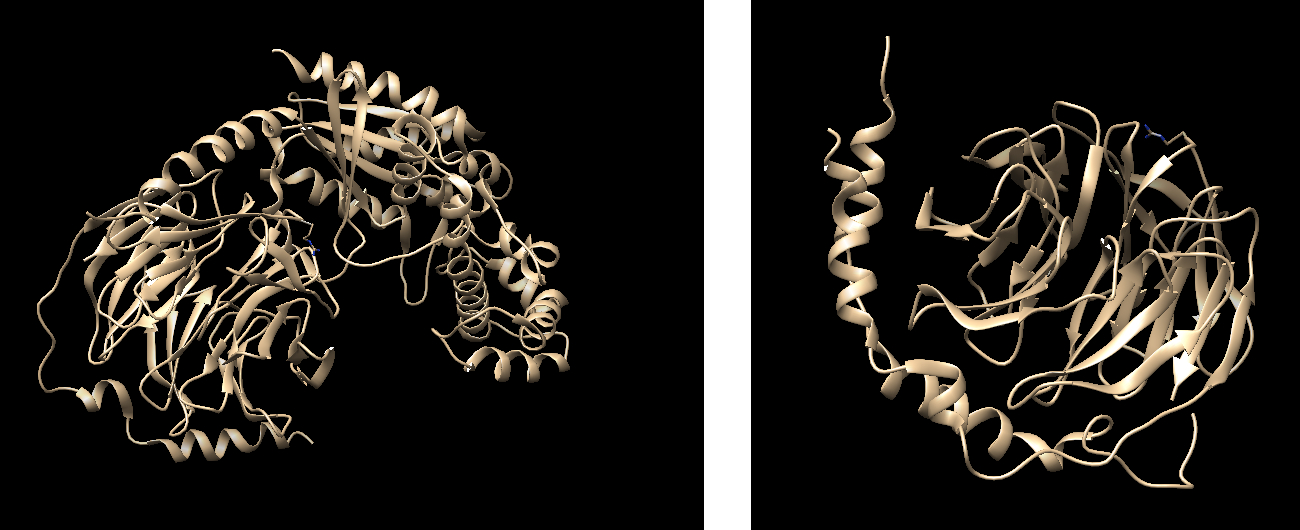
\includegraphics[width=0.8\textwidth]{hetero_before.jpg}
\caption{Subunits by pairs on a heterotrimeric G protein \href{https://www.rcsb.org/structure/3ah8}{(3AH8)}. On the left, interaction of chains A-B. On the right, interaction of chains B-G.}
\label{fig:1}
\end{figure}

\noindent
After running the program, the heterotrimeric G protein looks like que original PDB file. RMSD is 0, because is a toy model and fits perfectly.

\begin{figure}[h]
\centering
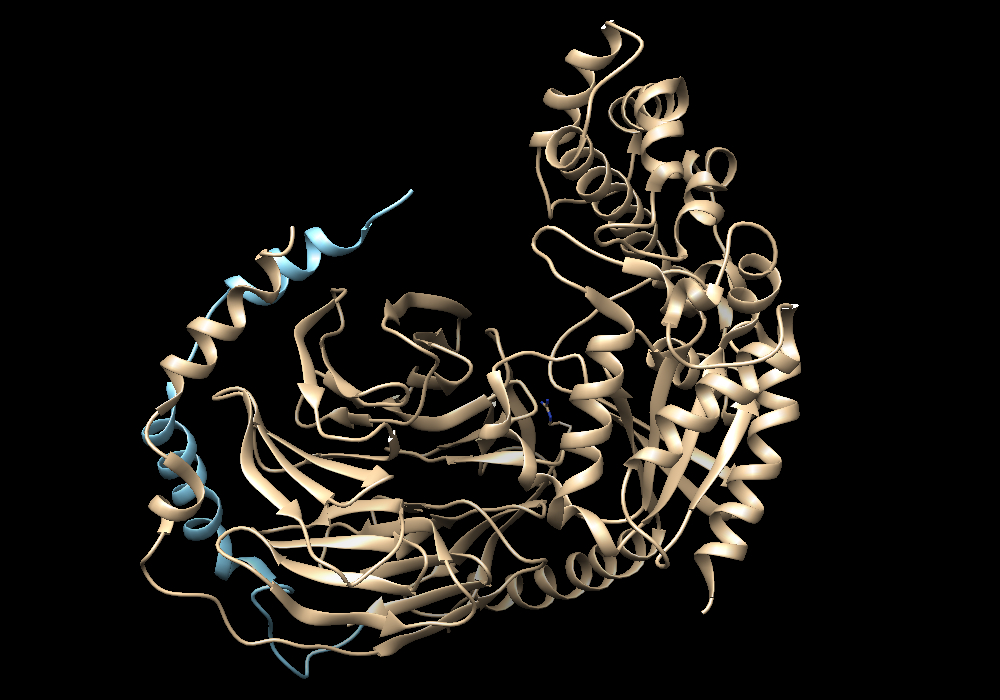
\includegraphics[width=0.8\textwidth]{hetero_after.jpg}
\caption{Complete structure of heterotrimeric G protein (3AH8), after running the program.}
\label{fig:2}
\end{figure}

\newpage

\subsection{Homodimer}

The example used for homodimers is the one provided by Professor Javier Garcia. This structure represents a nucleosome (and we were given the PDB files for interacting pairs of chains and those chains separatedly. We only use those interacting PDB files and NOT separated chains. There were 23 elements, homodimers and heterodimers repeated. Some of these interactions are represented in Figure~\ref{fig:3}.\\

\begin{figure}[h]
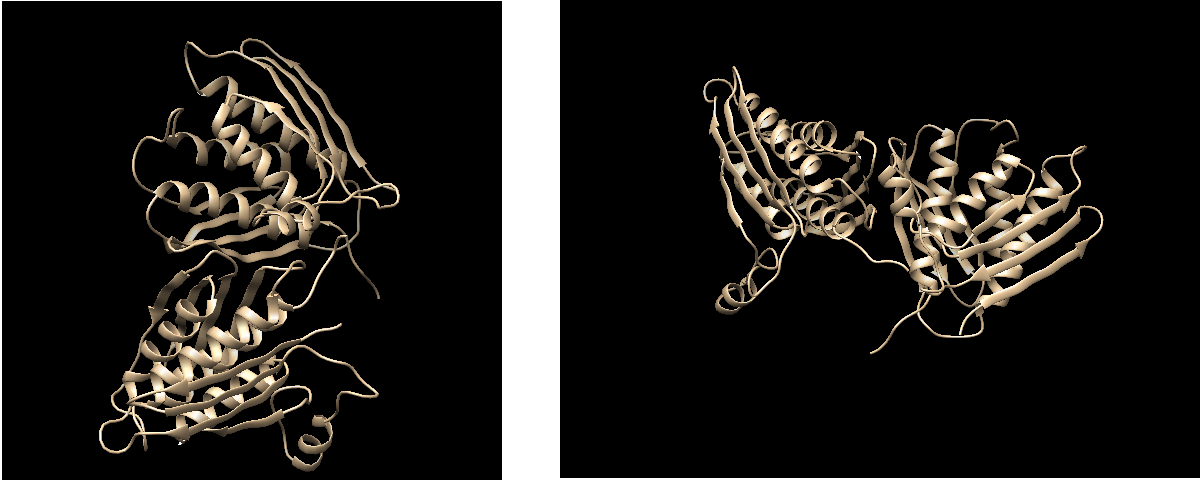
\includegraphics[width=0.8\textwidth]{homo_before.jpg}
\centering
\caption{Two examples of input files out of 23.}
\label{fig:3}
\end{figure}

\noindent
After running our program the final structure was the following (Figure~\ref{fig:4}).\\

\begin{figure}[h]
\centering
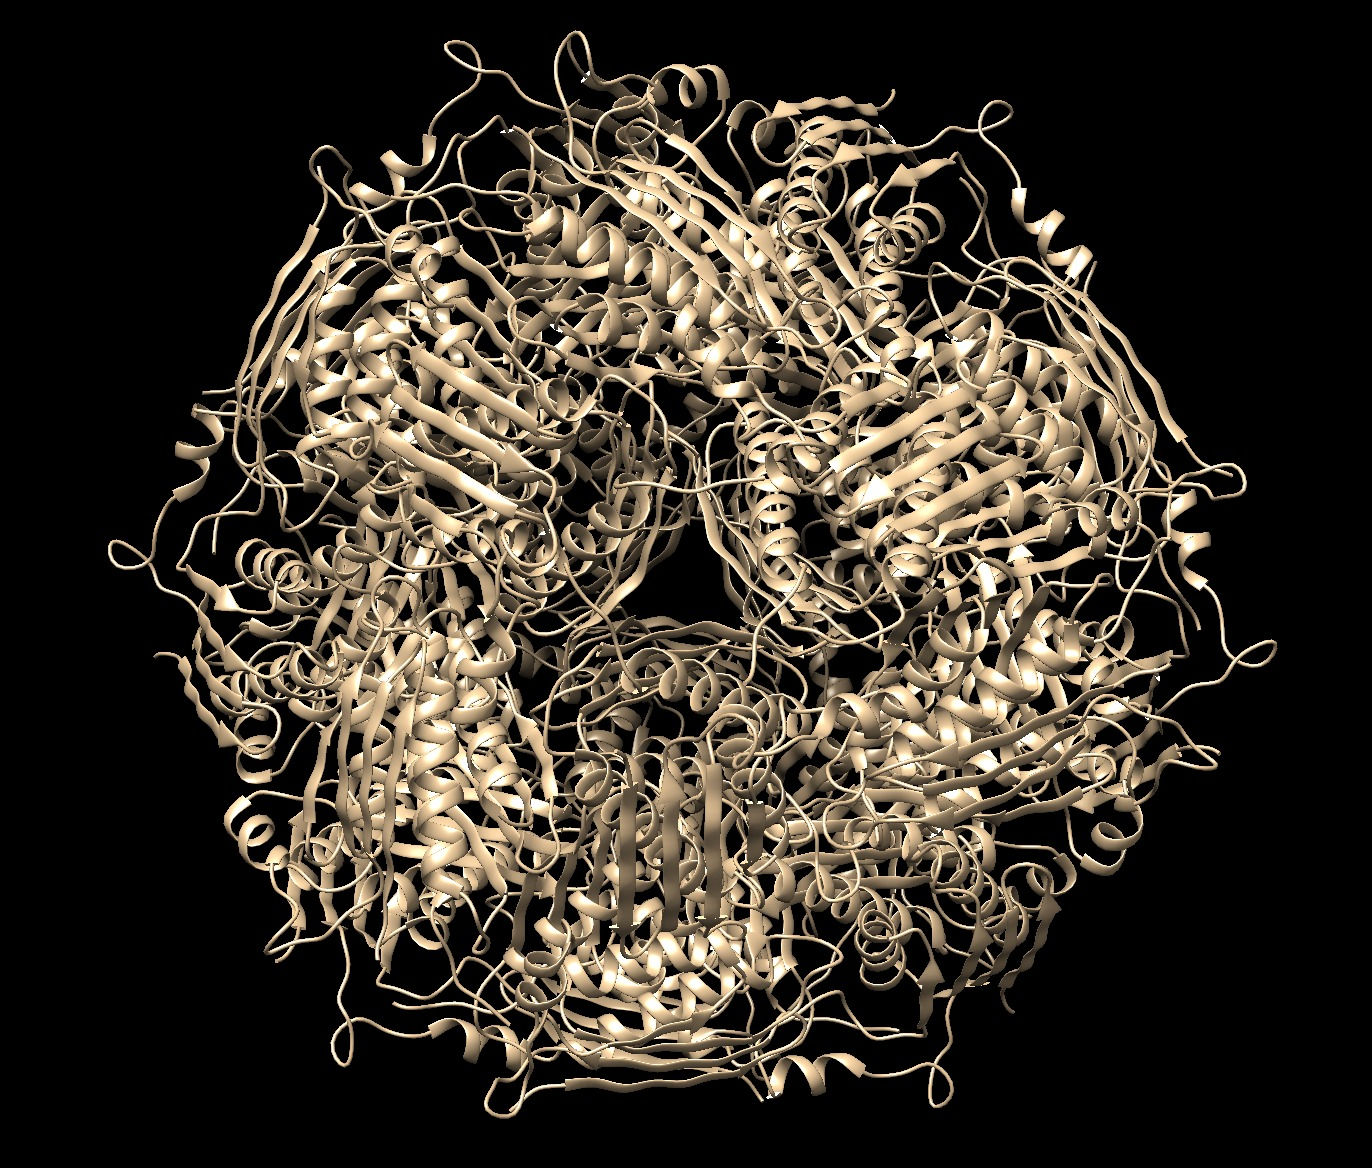
\includegraphics[width=0.8\textwidth]{homo_after.jpeg}
\caption{Final structure after running the program with the subunits given.}
\label{fig:4}
\end{figure}

\noindent
His3 is a gene of a nucleosome. Figure~\ref{fig:4} seems to be a complex nucleosome. At least, it has the proper shape. Therefore, although we do not know the real output, we can conclude that the program worked well.\\



\section{Generalisation of the program}

Generally, the program will work perfectly for non-repeated/normal heterodimers and heteropolimers defined as it was done.\\\\
For homodimers or repeated heterodimers it is more difficult, because a structural superimposition will not rebuild the whole structure. Moreover, we cannot know the correct orientation nor the stoichiometry. For these reasons, the program may fail recontructing this kind of structures.\\\\



\chapter{Discussion of the project}

In the project we had to understand and program usual algorithms in bioinformatics, such as sequence alignment and structural superimposition. It was a project that we were only told the title and we had to make up all the pipeline, the workflow, and the program.
If we were in a lab, we had a real problem, with a real project and with real data (data for training and data for testing). In this project, we had not had data to train or test and for these reason we may think that our program works perfectly and actually it could not be like this. With our own examples it worked, the program finished and created well the output, but at this point there is no guarantee that the program will work for any protein, with any input files. Personally, we believe that our program does what we want, we tested it and it worked and the pipeline is coherent and theoretically it must work.\\\\

\chapter{Conclusions}

This project have helped us to understand better concepts about structural superimposition, sequence alignment and python programming. In addition, we had to do the effort for create our own data and learn to use it. We did our best and we hope the program works.




\end{document}
